\subsubsection{Simulated rat hippocampal spike data in a navigation task}
\label{subsubsection:synthetic_results_details}

\paragraph{Dataset design.}
We simulate four place cells and 96 position-independent noise units for 600 s at 100 Hz, giving a $100\times60{,}000$ spike matrix. The signed Ornstein--Uhlenbeck movement model is motivated by \citet{theodoni_2018_theta_ou}. Position starts at 0.5 m on a 1-m track, with velocity
\begin{equation}
dv_t=\theta(\mu-v_t)\,dt+\sigma\,dW_t,\qquad
\theta=1\,\mathrm{s}^{-1},\quad\mu=0,\quad
\sigma=0.4\,\mathrm{m}\,\mathrm{s}^{-3/2},\quad v_0=0.
\end{equation}
Euler--Maruyama updates velocity before advancing position. At track endpoints, overshoot is reflected and velocity changes sign without damping. Motion uses NumPy's PCG64 generator with seed 42.

Cells 1--4 have centers $c=(0.2,0.4,0.7,0.7)$ m and amplitude parameters $a=(10,28,20,20)$ Hz. Their position-dependent firing rates are split Gaussians:
\begin{equation}
r_i(x)=0.1+a_i\exp\left[-\frac{1}{2}\left(\frac{x-c_i}{s_i(x)}\right)^2\right],\qquad
s_i(x)=\begin{cases}s_{i,L},&x<c_i,\\s_{i,R},&x\geq c_i.\end{cases}
\end{equation}
The left widths are $s_L=(0.05,0.10,0.14,0.06)$ m and right widths are $s_R=(0.10,0.05,0.14,0.06)$ m. All rates depend only on position, with no direction or velocity modulation (\autoref{figure:synthetic_rate_design}).

Each noise unit has a constant rate independently sampled from Uniform$(1,5)$ Hz. Spikes are independent Bernoulli draws with probability $r_i(x_t)\,dt$. Empirical rate maps divide spike counts by occupancy in 20 equal bins over the observed position range, including the maximum-position sample. Display smoothing uses a Gaussian standard deviation of 0.5 bins with nearest-edge extension. Exact generative maps are saved on a 501-point grid. Throughout this subsection, cells 1--4 correspond to zero-based unit IDs 0--3 in the saved artifacts; model seeds and latent indices remain zero-based.

\begin{figure}[tb]
    \centering
    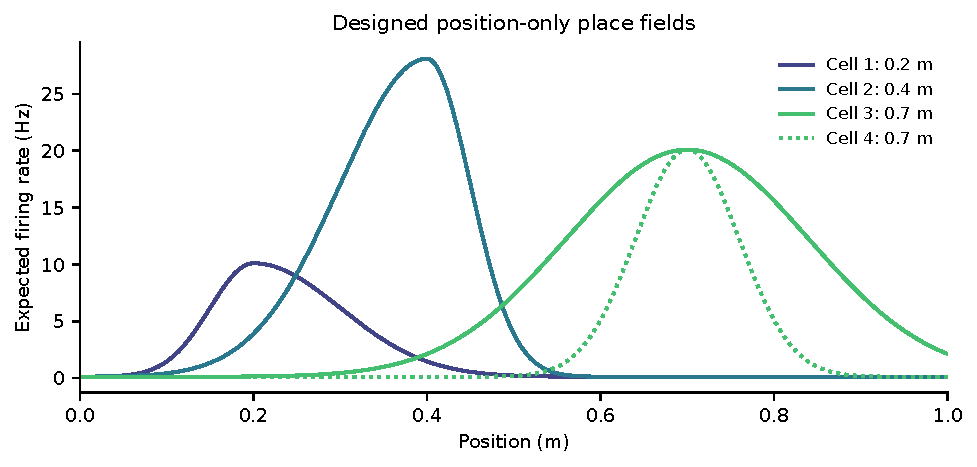
\includegraphics[width=0.72\linewidth]{figures/supplement_rate_design.pdf}
    \caption{\textbf{Synthetic place-field design.} Exact expected firing rates of the four place cells, including the 0.1-Hz baseline. Cells 1 and 2 have asymmetric tails; cells 3 and 4 share a center but differ in width. Colors indicate field center, and the dotted curve distinguishes cell 4 from cell 3.}
    \label{figure:synthetic_rate_design}
\end{figure}

\paragraph{FW-SED versus TW-SED.}
Full-recording reconstruction \metric{MSE} is $0.152\pm0.000$ for FW-SED and $0.153\pm0.000$ for TW-SED (mean $\pm1$ sample standard deviation across five initializations of each; standard deviations below 0.001 display as 0.000). Both architectures recover directional features under the same criteria, using the direction index (DI) and selection procedure defined below, though the TW-SED latents have higher selected composite direction scores. \autoref{figure:synthetic_temporal_comparison} compares the strongest passing forward feature from each architecture. These observations indicate TW-SED generates more interpretable latents for directionality in this dataset, though do not establish superiority of either architecture generally.

\paragraph{Oppositely directed temporal features.}
TW-SED finds features associated with ordered traversal of the first pair of place fields. We show the highest-scoring passing rightward feature (seed 0, latent 20) and leftward feature (seed 2, latent 66), using the selection criteria below. \autoref{figure:synthetic_temporal_features} shows each latent's place-cell decoder pattern alongside its 16 highest-activating nonoverlapping windows. Examples are selected greedily from all 11,981 windows with positive activation, without filtering position, displacement, reversals, or direction.

% Separate temporal comparison figures across successive pages.
\begin{figure}[!b]
    \centering
    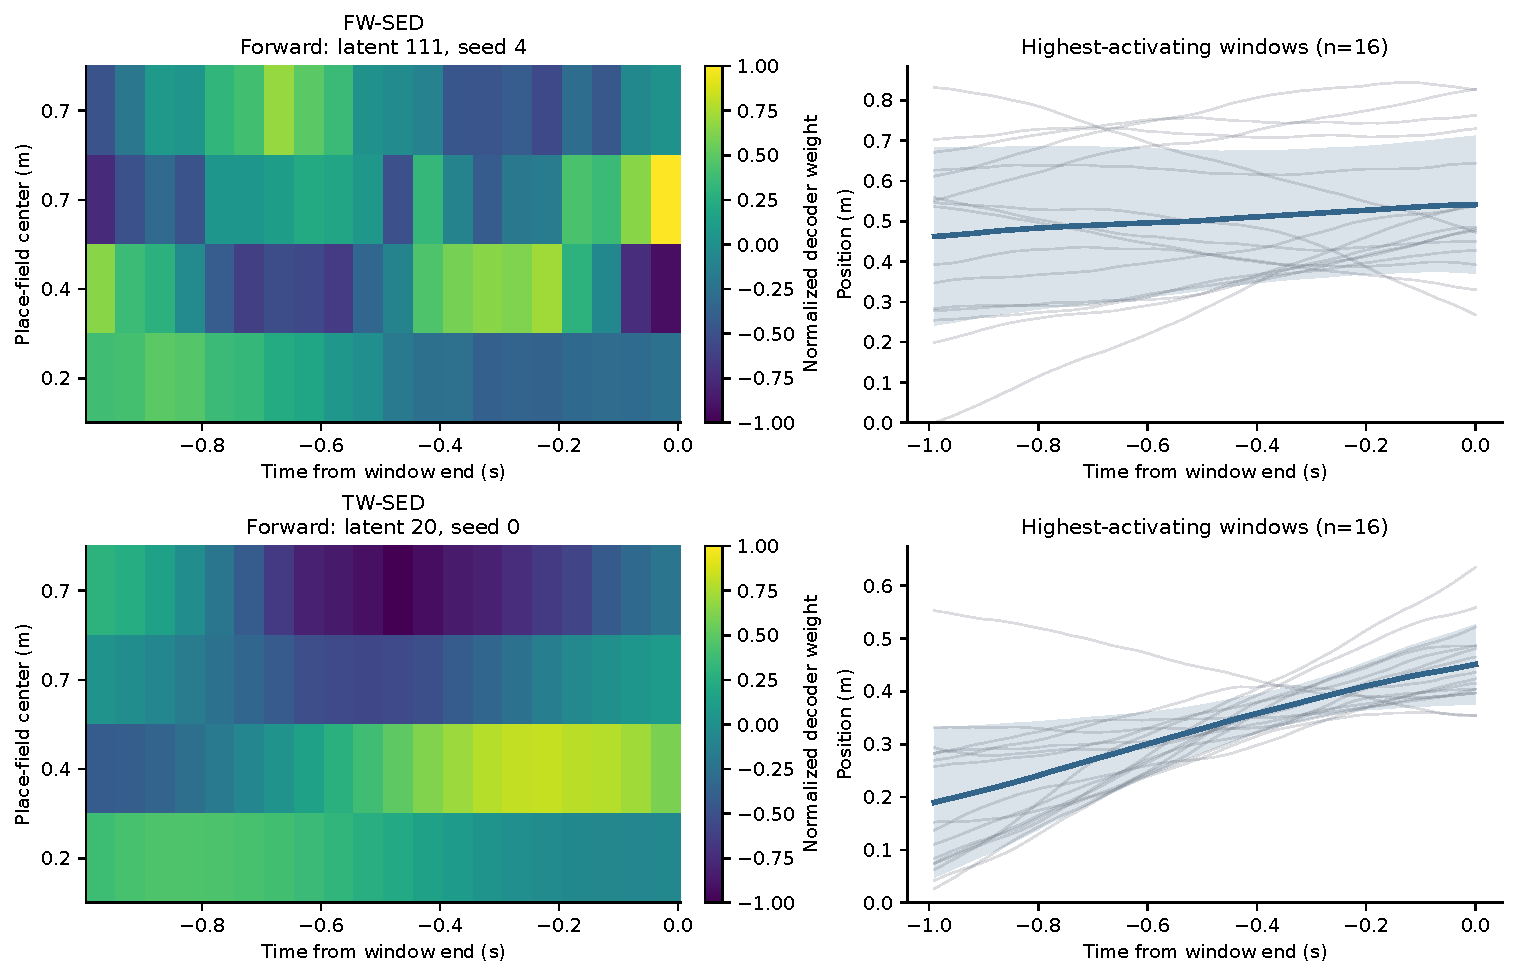
\includegraphics[width=\linewidth]{figures/supplement_temporal_comparison.pdf}
    \caption{\textbf{Comparison of FW-SED and TW-SED temporal features.} Top: strongest passing forward FW-SED latent; bottom: strongest passing forward TW-SED latent. Left panels show decoder weights for the four known place cells over the window, normalized by their maximum absolute weight. Right panels show the 16 highest-activating windows for each latent, selected without behavioral filtering. Thin curves are trajectories, the mean is emphasized, and shading is $\pm1$ sample standard deviation across trajectories. Both architectures use the same recording, window duration, latent count, sparsity, and training budget.}
    \label{figure:synthetic_temporal_comparison}

\end{figure}

\clearpage
\begin{figure}[!t]
    \centering
    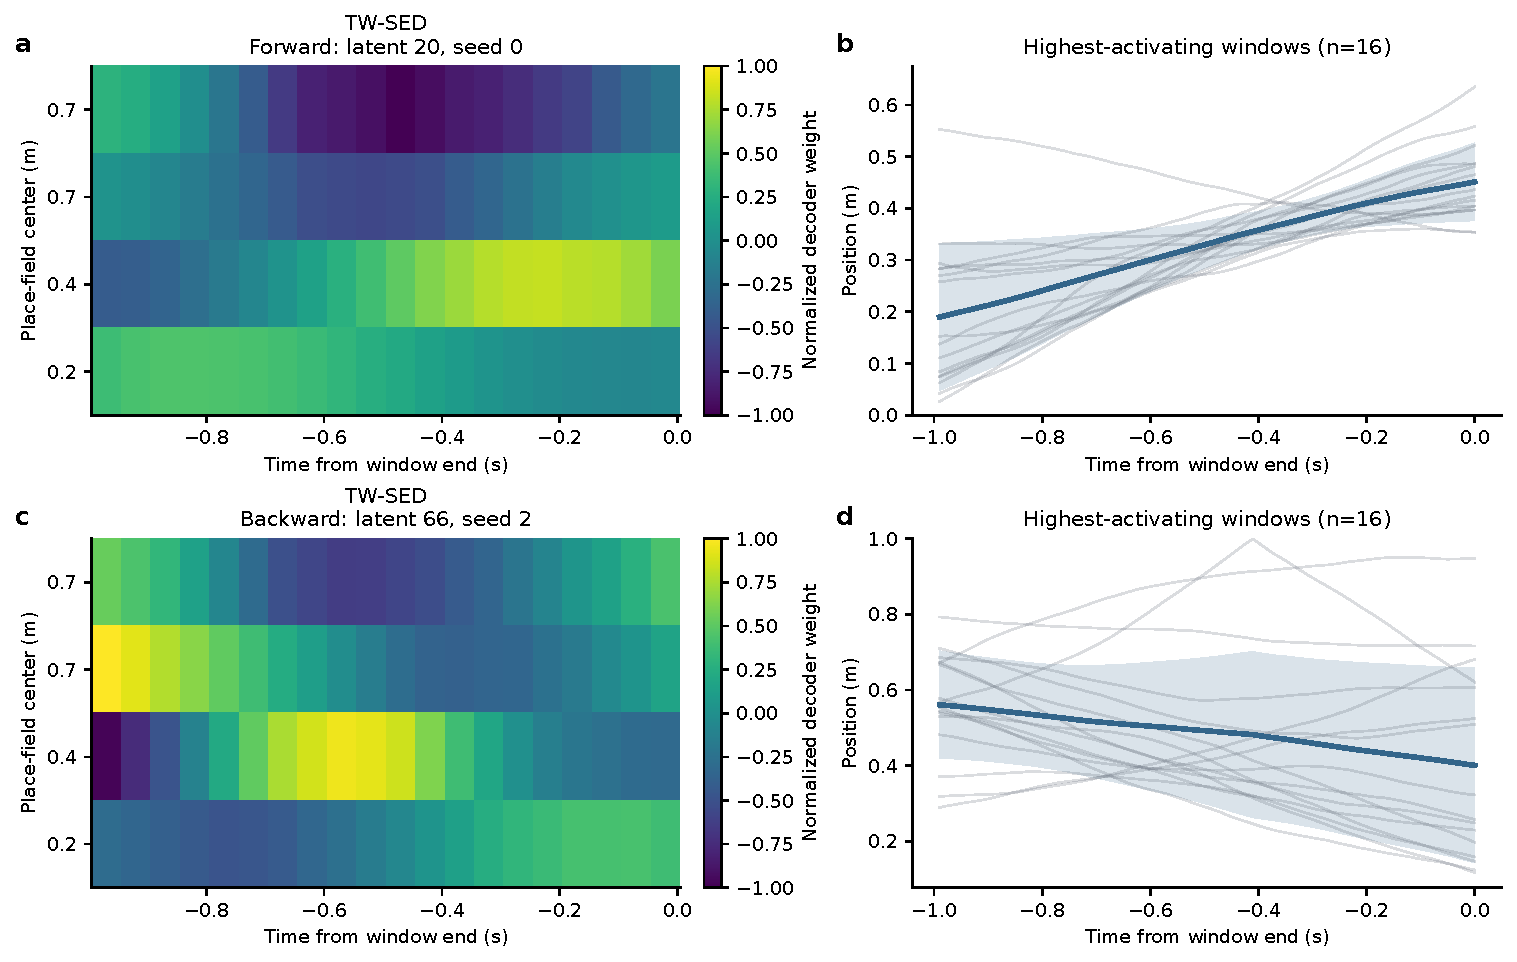
\includegraphics[width=\linewidth]{figures/supplement_temporal_features.pdf}
    \caption{\textbf{Rightward- and leftward-preferring TW-SED latents.} Left panels show decoder weights for the four known place cells over the window, normalized by their maximum absolute weight. Right panels show the 16 highest-activating windows for each latent, selected without behavioral filtering. Thin curves are trajectories, the mean is emphasized, and shading is $\pm1$ sample standard deviation across trajectories. The preferred direction occurs in 15/16 and 13/16 examples, respectively.}
    \label{figure:synthetic_temporal_features}
\end{figure}

\paragraph{Conditioning on clean crossings.}
To further examine traversals over the first pair of place fields, we restrict the eligible pool to strict nonreversing first-pair crossings with mean position in $[0.2,0.4]$ m, i.e. the animal's average position within the window must lie between 0.2 and 0.4 m, but its trajectory may extend beyond this interval. There are 218 rightward and 232 leftward eligible windows. Both directions compete when selecting the 16 highest-activating windows for each of the same two latents; no preferred-direction filter is applied. All examples per latent now follow its preferred direction (\autoref{figure:synthetic_ramp_conditioned}).

\paragraph{Source activity traceback for spatial latents.}
For each selected spatial latent in \autoref{figure:synthetic_results}c, we apply the \hyperref[paragraph:source_activity_traceback]{source activity traceback} to standardized unit activity in its same model input form: unique 50-ms binned counts. For the linear vanilla encoder, this multiplies each unit's activity by its encoder weight. We average equally over active bins within each of 20 equal position bins over the 1-m track, regardless of latent activation value. At each position, we then average equally across the selected runs with active bins there, retaining one curve per recorded unit (\autoref{figure:synthetic_unit_traceback}). Each field has five selected runs; a run contributes no value at positions where its latent never activates.

\paragraph{Source activity traceback over time.}
For the same two TW-SED latents in \autoref{figure:synthetic_temporal_features},  \autoref{figure:synthetic_temporal_coactivity} applies the \hyperref[paragraph:source_activity_traceback]{source activity traceback} to the same model input form: unstandardized 50-ms counts, retaining the unit and timebin axes across the full window. At each relative time, we then average these attributions equally across all windows with positive latent activation: 9,991 windows for the rightward latent and 7,281 for the leftward latent. This analysis does not restrict to clean crossings or top examples, and does not weight windows by activation value.

\clearpage
\begin{figure}[!t]
    \centering
    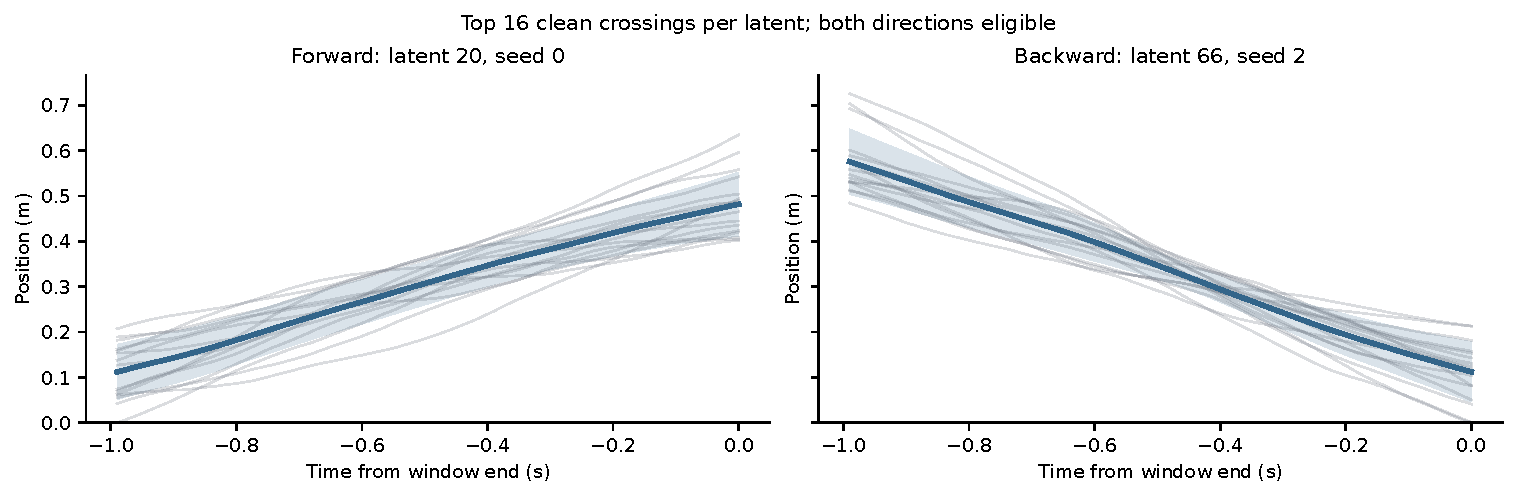
\includegraphics[width=\linewidth]{figures/supplement_ramp_conditioned.pdf}
    \caption{\textbf{The same temporal latents conditioned on clean first-pair crossings.} Left: seed 0, latent 20; right: seed 2, latent 66. Each panel contains its 16 highest-activating disjoint eligible crossings, with both directions competing. All 16 follow the respective preferred direction. Shading is $\pm1$ sample standard deviation across trajectories.}
    \label{figure:synthetic_ramp_conditioned}
\end{figure}

\begin{figure}[!b]
    \centering
    
\includegraphics[width=\linewidth]{figures/supplement_unit_traceback.pdf}
    \caption{\textbf{Source activity traceback for the spatial latents.} One panel per recovered place field shows each unit's mean encoder attribution (standardized activity times encoder weight) versus track position. Curves average active-bin attributions within 20 position bins, then average equally across the selected runs with observations in each bin. Shaded bands for place cells indicate $\pm1$ sample standard deviation across contributing runs. All 100 units are retained: place cells use the field-center color scale, cell 4 is dotted, and the 96 noise units are gray.}
    \label{figure:synthetic_unit_traceback}
\end{figure}

\clearpage
\begin{figure}[!t]
    \centering
    
\includegraphics[width=\linewidth]{figures/supplement_temporal_coactivity.pdf}
    \caption{\textbf{Source activity traceback over time for the two TW-SED latents.} Each curve is one unit's mean encoder attribution (50-ms count times the gradient of the latent's pre-activation) at each time within active windows. Left: seed 0, latent 20, using all 9,991 positive-activation windows; right: seed 2, latent 66, using all 7,281. Windows contribute equally, without behavioral filtering or activation weighting. Place cells use the field-center color scale, cell 4 is dotted, and the 96 noise units are gray.}
    \label{figure:synthetic_temporal_coactivity}
\end{figure}

\paragraph{Direction index.}
To measure a latent's preference for rightward or leftward movement, we compare its mean activation in the two directions:
\begin{equation}
\mathrm{DI}=
\frac{\bar z_{\mathrm{right}}-\bar z_{\mathrm{left}}}
{\bar z_{\mathrm{right}}+\bar z_{\mathrm{left}}+10^{-12}}.
\end{equation}
DI ranges from $-1$ to $1$: positive values indicate greater rightward activation, negative values greater leftward activation, and zero equal activation. Here, $\bar z_{\mathrm{right}}$ and $\bar z_{\mathrm{left}}$ are mean activations after matching the distribution of mean window position across directions, including windows in which the latent is inactive.

Matching position reduces differences caused by unequal sampling of locations. We group clean first-pair crossings by mean position into 0.025-m bins, retaining bins with at least ten windows in each direction. Within each bin, we calculate a mean activation for each direction. We then weight both means by the number of windows in the less frequent direction, giving greater influence to positions with more examples in both directions. The resulting mean for direction $d$ is
\begin{equation}
\bar z_d=\frac{\sum_{j\in\mathcal{J}}w_j\bar z_{j,d}}{\sum_{j\in\mathcal{J}}w_j},
\qquad w_j=\min(n_{j,\mathrm{right}},n_{j,\mathrm{left}}),
\end{equation}
where $\mathcal{J}$ contains the qualifying position bins, $n_{j,d}$ is the number of windows in bin $j$ for direction $d$, and $\bar z_{j,d}$ is their mean latent activation.

For clean crossings, eight position bins qualify, with weights summing to 209. To assess preference across the full track, we also analyze windows with no reversals and at least 0.1 m of net movement. The same procedure with wider, 0.1-m position bins retains eight bins, with weights summing to 939. Each total is the denominator for both directional means above. Both analyses use all windows in the retained bins, including overlapping windows, rather than only the illustrated examples.

\paragraph{Directional preferences.}
The two selected TW-SED latents show opposite preferences during clean crossings, with weaker preferences across the full track:
\begin{center}
\begin{tabular}{lrrrrr}
\toprule
& & & & \multicolumn{2}{c}{Preferred-direction examples} \\
TW-SED latent & Seed & Crossing DI & Full-track DI & \autoref{figure:synthetic_temporal_features} & \autoref{figure:synthetic_ramp_conditioned} \\
\midrule
20 (rightward) & 0 & $+0.558$ & $+0.118$ & $15/16$ & $16/16$ \\
66 (leftward) & 2 & $-0.479$ & $-0.199$ & $13/16$ & $16/16$ \\
\bottomrule
\end{tabular}
\end{center}
Neither latent activates exclusively in its preferred direction. These results support preferences for particular traversals, rather than uniform direction tuning throughout the recording.

\clearpage
\begin{figure}[!t]
    \centering
    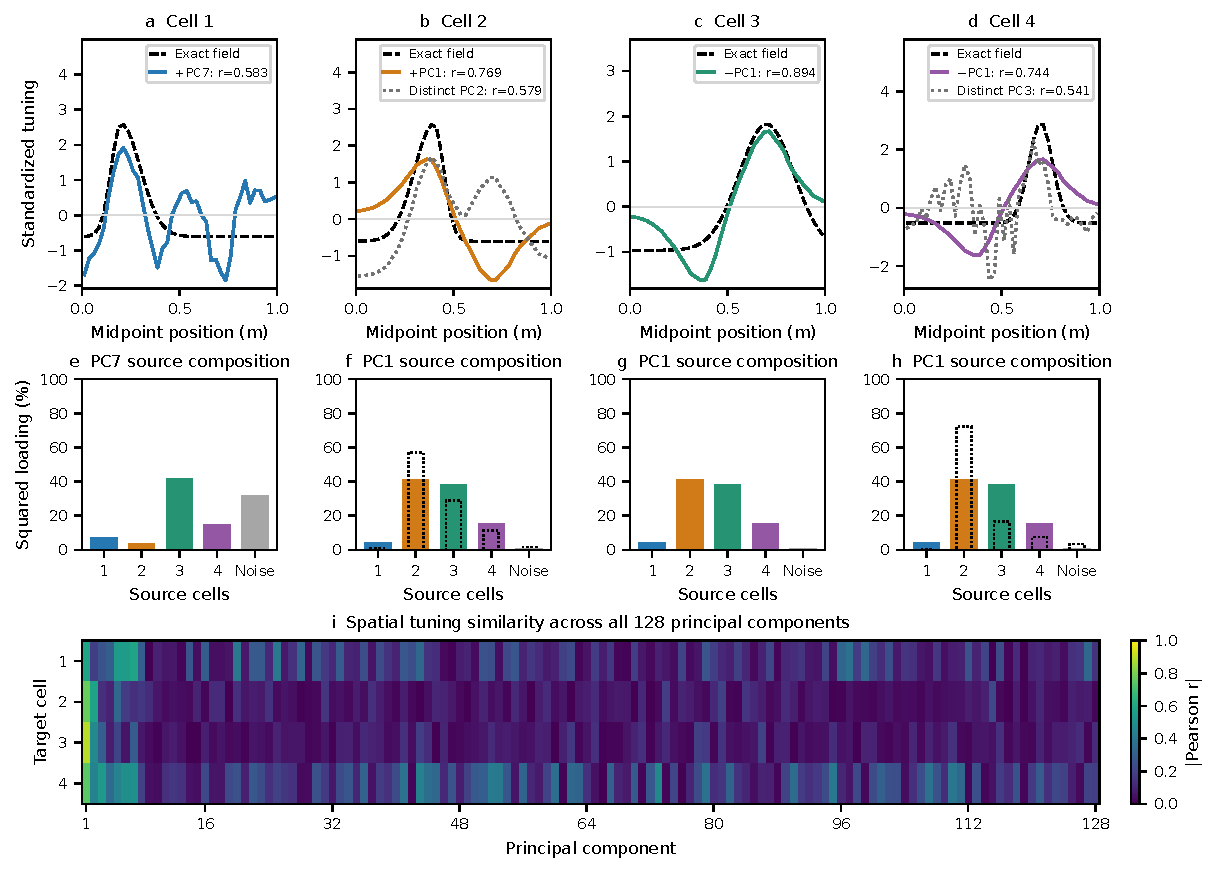
\includegraphics[width=\linewidth]{figures/supplement_pca_spatial.pdf}
    \caption{\textbf{Individual PCs cannot isolate place fields.} \textbf{(a--d)} Best independent PC matches to the four exact place fields. Each signed tuning curve and ground-truth curve is centered and scaled to unit standard deviation over spatial bins for display only. Gray dotted curves show the alternative when four distinct PCs are required. \textbf{(e--h)} Source composition of each best-matched PC, measured by squared loading. Dotted outlines show distinct-PC-assignment alternatives where applicable. \textbf{(i)} Absolute tuning correlations for all four place fields against each PC's spatial tuning curve.}
    \label{figure:synthetic_pca_spatial}
\end{figure}

\begin{figure}[!t]
    \centering
    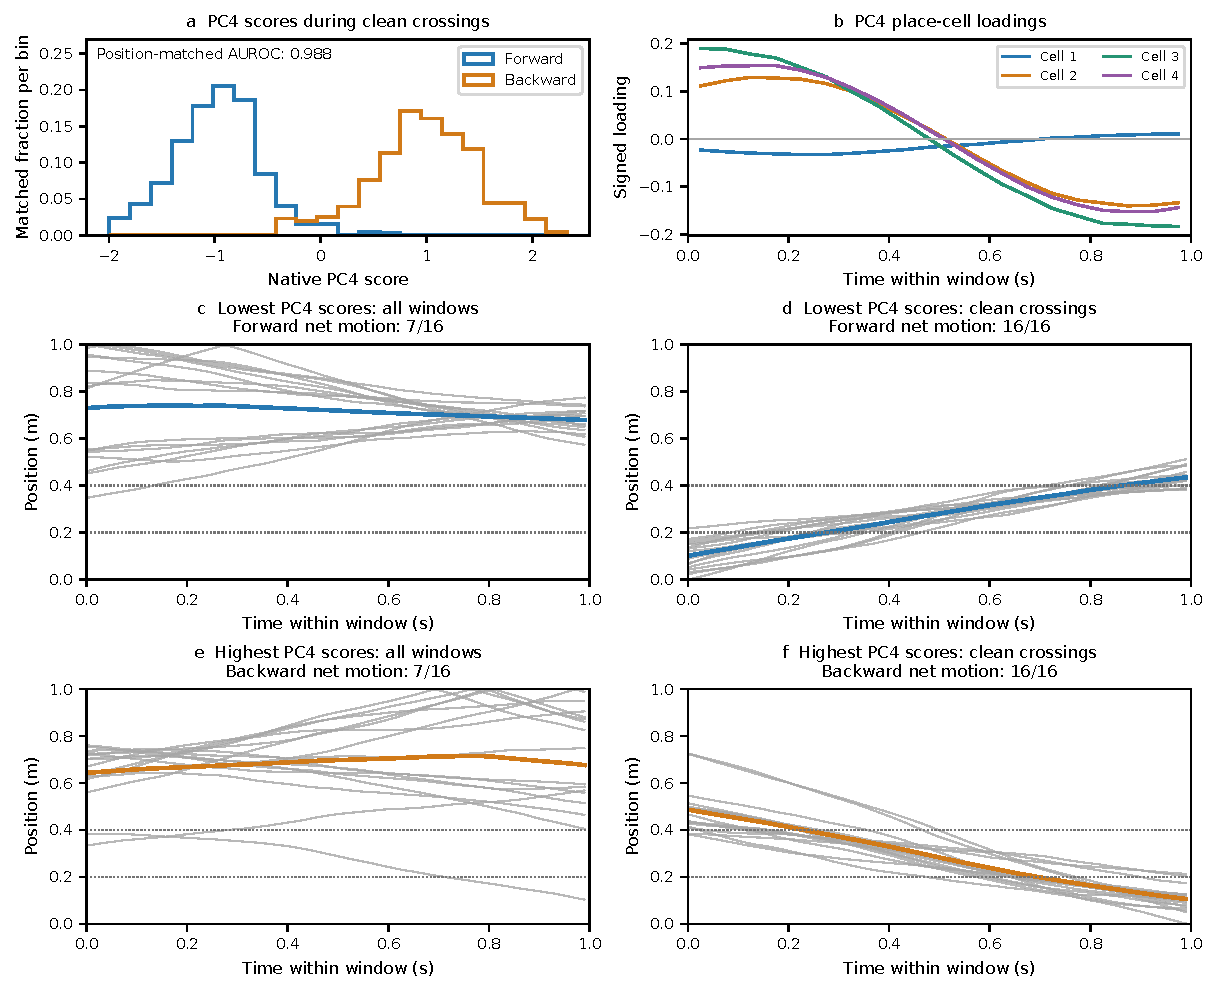
\includegraphics[width=\linewidth]{figures/supplement_pca_direction.pdf}
    \caption{\textbf{PC4 distinguishes traversal direction within clean crossings.} (\textbf{a}) Native PC score distributions for forward and backward clean crossings, reweighted to match mean-position occupancy. Lower scores favor forward motion within crossings, and higher scores favor backward motion. (\textbf{b}) PC4's signed weights for the four place cells at each time within the window. Cells 2--4 have positive weights early and negative weights late, revealing an early-versus-late activity contrast shared across several place cells. \textbf{c--f:} The 16 lowest (c,d) or highest (e,f) score windows, selected either from the full recording (c,e) or only clean first-pair crossings (d,f). Gray curves show individual nonoverlapping trajectories; colored curves show their means.}
    \label{figure:synthetic_pca_direction}
\end{figure}

\paragraph{Windowed PCA baseline.}
We fit PCA to the same complete 600-s recording and 1-s windows used by the W-SEDs, retaining 128 principal components to match their latent count, $D=128$. Each window contains 20 timebins across 100 neurons, which we flatten into a vector of 2,000 values, in ``time-then-neuron'' order, preserving temporal order. Sliding the window forward in 50-ms steps gives 11,981 windows and an input matrix $X\in\mathbb{R}^{11{,}981\times2{,}000}$, with one row per window. We mean-center each column without scaling its variance and fit PCA using a full singular value decomposition. The retained components explain 15.645\% of the centered input variance. We use the resulting component scores for both spatial and directional analyses.

To describe each PC's spatial tuning, we assign each window a position by averaging the animal's position at its two central 10-ms samples. We divide the 1-m track into 40 equal spatial bins and average the signed PC scores of windows assigned to each bin:
\begin{equation}
\label{eq:pca_spatial_tuning}
T_{p,j}=\frac{1}{|\mathcal{W}_j|}\sum_{w\in\mathcal{W}_j}z_{w,p}.
\end{equation}
Here, $z_{w,p}$ is the signed score of PC $p$ in window $w$, $\mathcal{W}_j$ is the set of windows assigned to spatial bin $j$, and $|\mathcal{W}_j|$ is their number. The 40 values $T_{p,j}$ form the PC's spatial tuning curve.

We compare this PC spatial tuning curve with each known place field using absolute Pearson correlation. Taking the absolute value treats positively and negatively correlated patterns as equally strong matches, since a PC's sign is arbitrary. Computing $C_{i,p}$ for all four fields and 128 PCs gives the $4\times128$ correlation matrix in \autoref{figure:synthetic_pca_spatial}i.

Independent best matches for place cells 1--4 are $+$PC7, $+$PC1, $-$PC1, and $-$PC1, with correlations 0.583, 0.769, 0.894, and 0.744. Here three targets reuse the same component; requiring four distinct components gives PCs 7, 2, 1, and 3, with correlations 0.583, 0.579, 0.894, and 0.541. The best spatial matches do not cleanly isolate any individual place field: they retain additional peaks, contrasts between locations, or mixed source contributions (\autoref{figure:synthetic_pca_spatial}).

Interestingly, PC4 strongly distinguishes forward from backward movement among the same clean first-pair crossings used above (\autoref{figure:synthetic_pca_direction}). To compare directions at similar locations, we group crossings by mean position into 0.025-m bins, retaining bins with at least ten windows in each direction. Within each bin, we calculate how well the signed PC scores distinguish forward from backward crossings using \metric{AUROC}. We then average these values, weighting each bin by its less frequent direction count. This gives greater influence to locations with more examples in both directions and reduces confounding from differences in where forward and backward crossings occur. The weighted average is
\begin{equation}
\label{eq:pca_position_matched_auroc}
A=\frac{\sum_{j\in\mathcal{J}}w_j\,\metric{AUROC}_j}{\sum_{j\in\mathcal{J}}w_j},
\qquad w_j=\min(n_{j,\mathrm{forward}},n_{j,\mathrm{backward}}),
\end{equation}
where $\mathcal{J}$ contains the qualifying position bins, $\metric{AUROC}_j$ is the direction AUROC within bin $j$, and $n_{j,\mathrm{forward}}$ and $n_{j,\mathrm{backward}}$ count its forward and backward windows. We report $\max(A,1-A)$ to account for PCA's arbitrary sign, using one sign orientation across all bins. PC4 achieves a position-matched \metric{AUROC} of 0.988 after this averaging, and has lower native PC scores favoring forward crossings and higher PC scores favoring backward crossings.
